\documentclass[11pt, a4paper, titlepage]{article}
\title{Testing}
\usepackage{graphicx}
\usepackage{titlesec}
\usepackage{geometry}
\newgeometry{margin=3cm}
%\setlength{\parskip}{1em}
\usepackage{url}
\usepackage[none]{hyphenat}
\usepackage{subcaption}
\usepackage{sectsty}
\usepackage{listings}
\subsectionfont{\small}
\begin{document}

\begin{center}
{\Large \textbf{COMP6208 Advanced Machine Learning\\Research Final Report}}\\
\vspace{0.7cm}
University of Southampton\\
School of Electronics and Computer Science\\
Friday 13\textsuperscript{th} February, 2015\\
\vspace{0.7cm}
Team \textbf{{\large Seahorse}}\\
Alexander Ally (aa2g11)\\
Hendrik Appel (hja1g11)\\
Samir Moussa (sm28g11)
\end{center}

\section{Introduction}

\section{Preprocessing and Feature Extraction}
Since the trips were merely composed from sequences of GPS co-ordinates taken at one second intervals the data had to be processed and features designed and extracted before machine learning techniques could be applied to make predictions. Additionally the gps co-ordinates given in the data are subject to inaccuracy. 

\subsection{Smoothing the Data}
Because the features were often based upon first and second order gradients of the original data, noise caused a lot of problems. Particularly when the speed of the vehicle was low, small fluctuations in the position of the vehicle caused a small velocity and acceleration to be reported. When directional information is extracted from these gradients (and magnitude information thrown away) there would appear to be wild changes in direction when really the vehicle was stationary and there was small fluctuations in the position information being reported. 

In order to solve this problem a number of different avenues were explored. One simple approach was report any velocity with a magnitude of less than a small value to be set to 0. However this ignored smoothness issues that occurred at higher speeds. To remedy this a simple filter was constructed by applying the Discrete Fourier Transform and reconstructing th data using fewer components. This does appear to work well in general but in sections where the driver is crawling along at a very low speed were the filter wrongly assumes that the driver is stationary. This can be observed in the plot in figure \ref{fig:fouriersmooth}.

\begin{figure}
    \center
    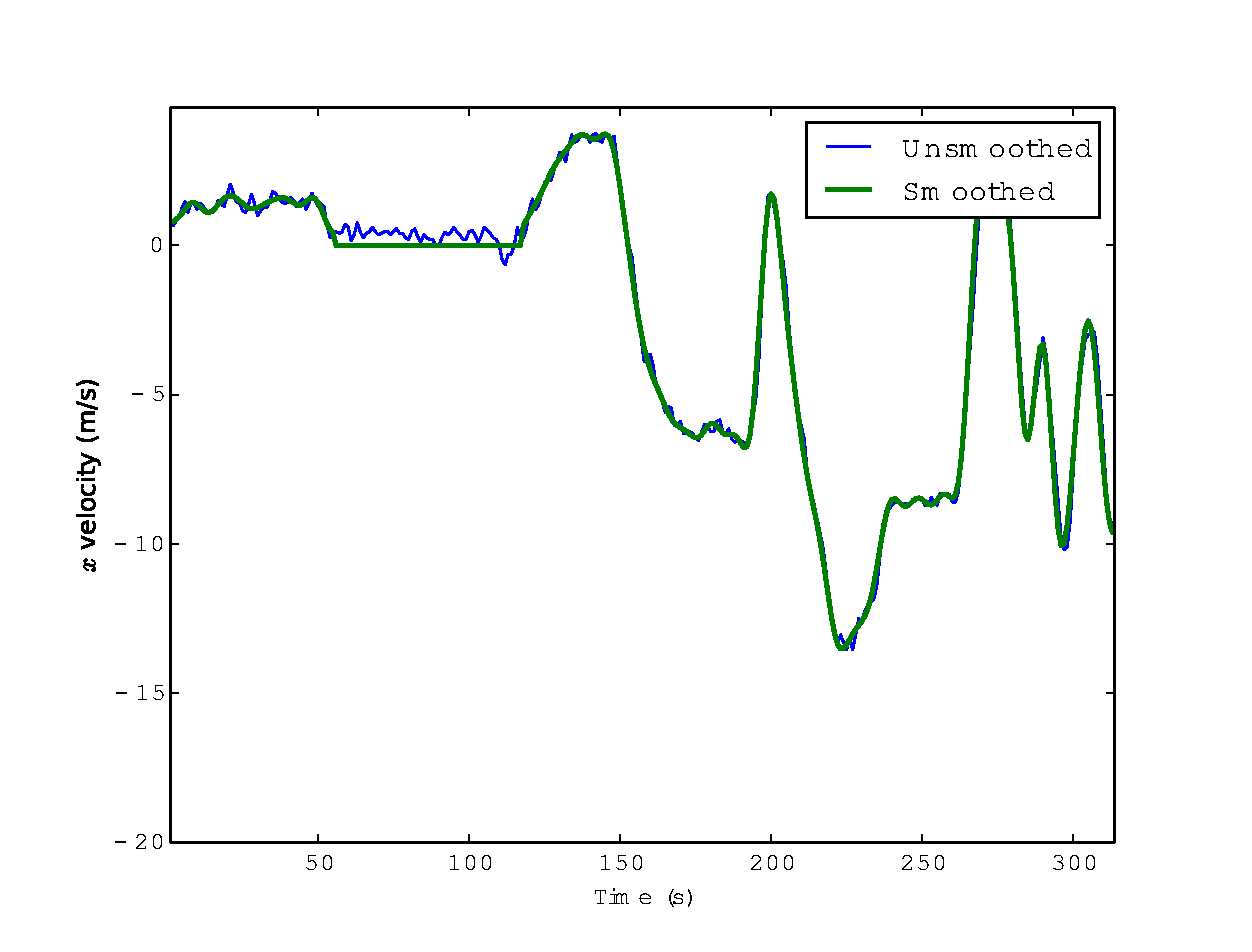
\includegraphics[scale=0.6]{fouriersmooth}
    \caption{Fourier smoothed velocity component}
    \label{fig:fouriersmooth}
\end{figure}

Another approach attempted was to apply the Savitzky-Golay filter to smooth the data. Savitzky-Golay smooths data by convolution, fitting a polynomial to successive windows over the data points using a least squares optimisation. One can see that in figure \ref{fig:savgolsmooth} that the problem of threshold smoothing is does not appear and that the data appears to be much smoother. However some jaggedness remains in periods of low velocity.

\begin{figure}
    \center
    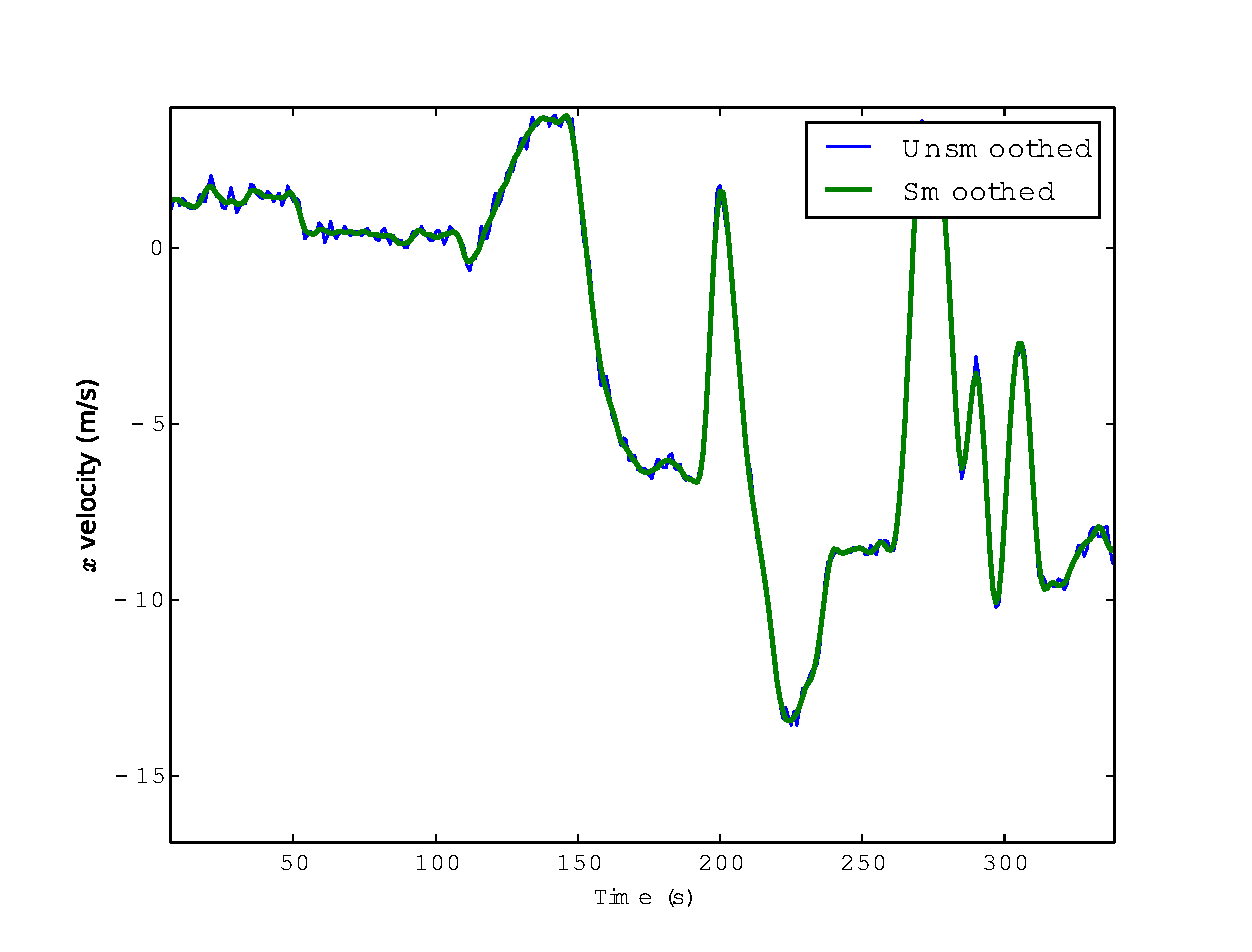
\includegraphics[scale=0.6]{savgolsmooth}
    \caption{Savitzky-Golay smoothed velocity component}
    \label{fig:savgolsmooth}
\end{figure}

\subsection{Feature Extraction}

\end{document}
